\documentclass{beamer}
\usetheme{metropolis}

\usepackage[utf8]{inputenc}
\usepackage[T1]{fontenc}
\usepackage[french]{babel}
\usepackage{listings}
\usepackage{graphicx}
\usepackage{hyperref}
\usepackage{xcolor}
\usepackage{svg}
\usepackage{tikz}
\usetikzlibrary{positioning, arrows.meta, decorations.markings}
% Define custom colors
\definecolor{commentgray}{rgb}{0.5, 0.5, 0.5}
\definecolor{keywordorange}{rgb}{0.8, 0.4, 0.0}
\definecolor{typeblue}{rgb}{0.2, 0.6, 1.0}
\definecolor{fggray}{rgb}{0.4, 0.4, 0.4}


\title{Mettre un titre original}
\author{Étienne Collin, Emeric Laberge}
\date{\today}

\begin{document}

\maketitle

\begin{frame}{Plan de la présentation}
	\tableofcontents
\end{frame}
\section{Introduction}
\begin{frame}{Introduction}

\end{frame}

\section{Contexte et Objectifs}
\begin{frame}{Contexte et Objectifs}

\end{frame}

\section{Description du Protocole HDLC}
\begin{frame}{Description du Protocole HDLC}
  \textbf{High-Level Data Link Control} (HDLC) est un protocole de communication
  de données qui opère au niveau de la couche liaison du modèle OSI.\\ 
  Il est utilisé pour la transmission de données entre machines distantes.\\ 
  Dans ce projet, nous allons implémenter une version simplifiée du protocole
  HDLC en utilisant le langage de programmation \textbf{Rust}. 
\end{frame}

\section{Architecture du Projet}
\begin{frame}{Architecture du Projet} 
  Dans notre projet, nous avons deux composantes principales : l'\textbf{émetteur}
  représenté par le client  et le \textbf{récepteur} représenté
  par le serveur.\\
  L'émetteur est responsable de l'envoi des trames et le récepteur est
  responsable de la réception des trames.\\ 
  Nous avons également une troisième composante qui est l'intermédiaire de
  simulation qui est responsable de simuler les erreurs de transmission. Dans
  notre cas, c'est le \textbf{tunnel} qui est responsable de cette tâche. 
\end{frame}

\begin{frame}{Visualisation simplifiée de l'architecture}
  
  \begin{tikzpicture}[scale=0.8, node distance=4cm]
    % Nodes
    \node (client) [draw, rectangle] {Client};
    \node (tunnel) [draw, rectangle, right of=client] {Tunnel};
    \node (server) [draw, rectangle, right of=tunnel] {Serveur};
    \node[below of=tunnel, yshift=2cm] (lost) [draw, rectangle,dashed]{Trame perdue};

    % font size to small
    \tiny

    % Arrows
    % Lost frame annotation
    \path[->] (client.north east) edge[bend left=45] node[fill=white] {Envoie de
      trame}(tunnel.north west);
    \path[->] (tunnel.north east) edge[bend left=45] node[fill=white] {Réception
      de trame}(server.north west);
    \path[->] (server.south west) edge[bend left=45] node[fill=white]
      {Envoie de trame}(tunnel.south east);
    \path[->] (tunnel.south west) edge[bend left=45] node[fill=white] {Réception
      de trame}(client.south east);
    \path[dashed,->] (tunnel) edge[] node[fill=white] {Perte de trame} (lost);
    \draw[dashed,->] (tunnel) [loop above] to node {Bit flip} (tunnel);
    \path[->] (server) edge[loop right] node {ACK}(server);
\end{tikzpicture}
\end{frame}

\begin{frame}{Architecture détaillée}
  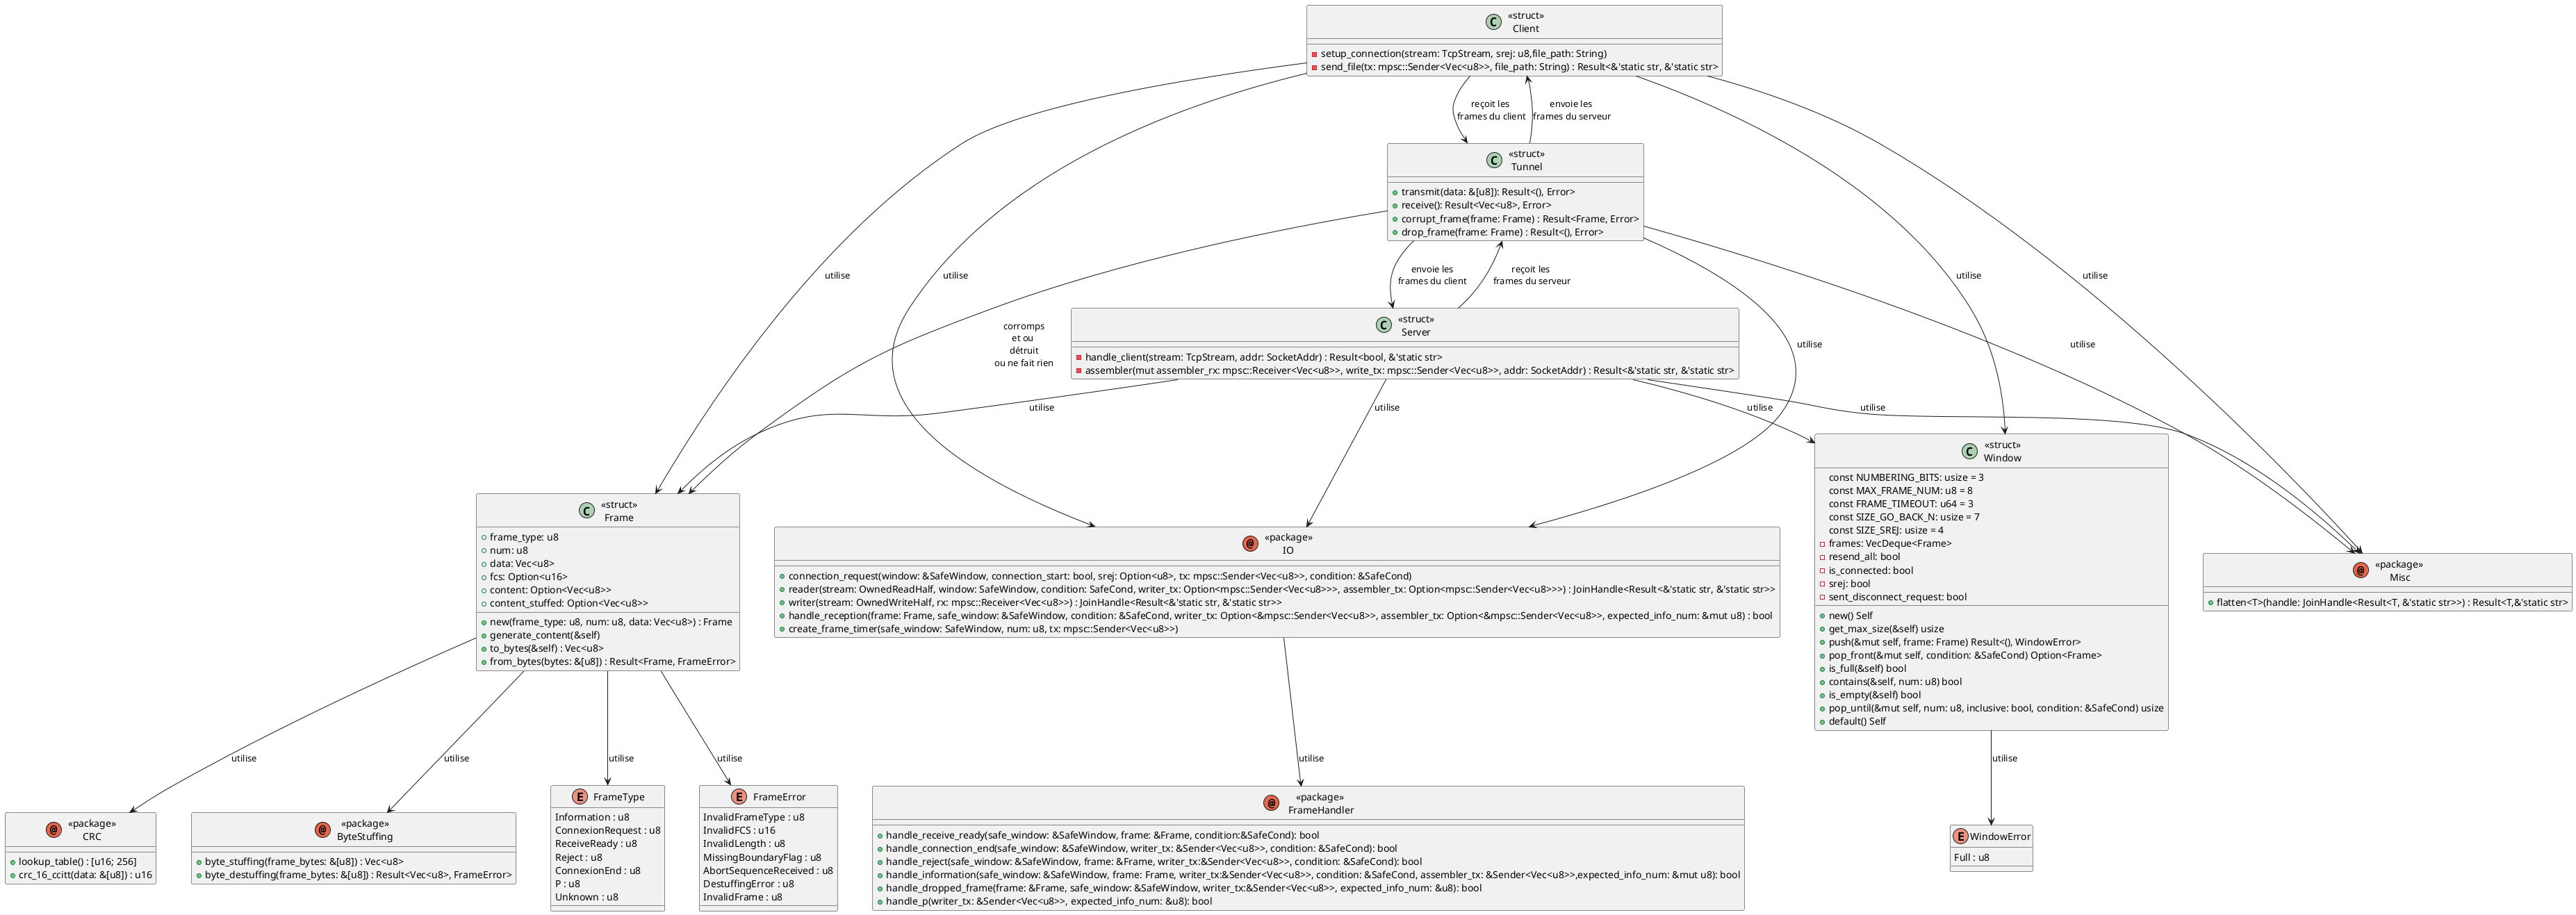
\includegraphics[width=\textwidth,border=1px]{../class-diagram/class-diagram}
\end{frame}

\section{Fonctionnalités de l'Émetteur}
\begin{frame}{Fonctionnalités de l'Émetteur}
  Les fonctionnalités de l'émetteur sont les suivantes : 
  \begin{itemize}
    \item Établissement de la connexion 
    \item Séparation des données en trames 
    \item Gestion de la fenêtre d'envoi
    \item Byte stuffing 
    \item Byte destuffing
    \item Envoi de trames
    \item Attente de l'acquittement
    \item Vérification de l'intégrité des données 
    \item Gestion des erreurs ou des pertes de trames 
    \item Fermeture de la connexion
  \end{itemize}
\end{frame}

\begin{frame}{Établissement de la connexion}
\end{frame}

\begin{frame}{Séparation des données en trames} 
\end{frame}

\begin{frame}{Gestion de la fenêtre d'envoi} 
\end{frame} 

\begin{frame}{Byte stuffing} 
\end{frame}

\begin{frame}{Byte destuffing}
\end{frame}

\begin{frame}{Envoi de trames} 
\end{frame} 


\begin{frame}{Attente de l'acquittement} 
\end{frame} 
\begin{frame}{Vérification de l'intégrité des données} 
\end{frame}

\begin{frame}{Gestion des erreurs ou des pertes de trames} 
\end{frame}

\begin{frame}{Fermeture de la connexion} 
\end{frame}




\section{Fonctionnalités du Récepteur}
\begin{frame}{Fonctionnalités du Récepteur}
  Les fonctionnalités du récepteur sont les suivantes : 
  \begin{itemize}
    \item Établissement de la connexion 
    \item Réception de trames
    \item Gestion de la fenêtre de réception
    \item Byte stuffing 
    \item Byte destuffing
    \item Envoi d'acquittements
    \item Vérification de l'intégrité des données 
    \item Gestion des erreurs ou des pertes de trames 
    \item Fermeture de la connexion
  \end{itemize}

\end{frame}

\begin{frame}{Établissement de la connexion}
\end{frame}

\begin{frame}{Réception de trames}
\end{frame}

\begin{frame}{Gestion de la fenêtre de réception}
\end{frame}

\begin{frame}{Byte stuffing} 
\end{frame}

\begin{frame}{Byte destuffing}
\end{frame}

\begin{frame}{Envoi d'acquittements}
\end{frame}

\begin{frame}{Vérification de l'intégrité des données}
\end{frame}

\begin{frame}{Gestion des erreurs ou des pertes de trames}
\end{frame}

\begin{frame}{Fermeture de la connexion}
\end{frame}

\section{Fonctionnalités du Tunnel}
\begin{frame}{Fonctionnalités du Tunnel}
  Les fonctionnalités du tunnel sont les suivantes : 
  \begin{itemize}
    \item Simulation des erreurs de transmission
    \item Simulation des pertes de trames
  \end{itemize}
\end{frame}

\begin{frame}{Simulation des erreurs de transmission}
\end{frame}

\begin{frame}{Simulation des pertes de trames}
\end{frame}

\section{Gestion des Erreurs}
\begin{frame}{Gestion des Erreurs}
  Les erreurs de transmission peuvent être de plusieurs types : 
  \begin{itemize}
    \item Erreur de CRC (causé par un bit flip)
    \item Perte de trame
  \end{itemize}
\end{frame}
\begin{frame}{CRC} 
\end{frame}
\begin{frame}{Perte de trame} 
\end{frame}



\section{Calcul du CRC}
\begin{frame}{Calcul du CRC}

\end{frame}

\section{Bit Stuffing}
\begin{frame}{Bit Stuffing}

\end{frame}

\section{Tests et Simulations}
\begin{frame}{Tests et Simulations}

\end{frame}

\section{Conclusion}
\begin{frame}{Conclusion}

\end{frame}

\section{Questions et Réponses}
\begin{frame}{Questions et Réponses}

\end{frame}
\end{document}
